\subsection*{Problema 02}

\noindent\textbf{Enunciado:} 
Probar que si $x < 1$ (con $x > 0$), entonces se cumple que $\ln(x) < x$.

\noindent\textbf{Solución:}
Para demostrar la desigualdad propuesta, definimos una función auxiliar en todo el dominio $x > 0$ tal que:

\begin{align*}
    f(x) &= x - \ln(x)
\end{align*}

El objetivo es analizar el comportamiento de esta función y determinar su valor mínimo absoluto para $x > 0$. Para ello, calculamos la primera derivada de $f(x)$ respecto a $x$:

\begin{align*}
    f'(x) &= \dfrac{d}{dx} \left[ x - \ln(x) \right] \\
    f'(x) &= 1 - \dfrac{1}{x}
\end{align*}

Igualamos la derivada a cero para encontrar los puntos críticos en el dominio $x > 0$:

\begin{align*}
    1 - \dfrac{1}{x} &= 0 \\
    1 &= \dfrac{1}{x} \\
    x &= 1
\end{align*}

El único punto crítico ocurre en $x = 1$. Evaluamos la segunda derivada para determinar la naturaleza de este punto crítico:

\begin{align*}
    f''(x) &= \dfrac{d}{dx} \left[ 1 - \dfrac{1}{x} \right] \\
    f''(x) &= \dfrac{1}{x^2}
\end{align*}

Evaluando en el punto crítico $x = 1$:

\begin{align*}
    f''(1) &= \dfrac{1}{(1)^2} = 1 > 0
\end{align*}

Dado que la segunda derivada es positiva en $x = 1$, por el criterio de la segunda derivada, $f(x)$ tiene un mínimo absoluto en dicho punto. Calculamos el valor de la función en este mínimo:

\begin{align*}
    f(1) &= 1 - \ln(1) \\
    f(1) &= 1 - 0 = 1
\end{align*}

Como $f(1) = 1$ es el valor mínimo de la función para todo $x > 0$, se concluye que la función es estrictamente positiva en todo su dominio:

\begin{align*}
    f(x) &\ge 1 > 0 \quad \text{para todo } x > 0
\end{align*}

Sustituyendo la definición original de $f(x)$, obtenemos:

\begin{align*}
    x - \ln(x) &> 0 \\
    x &> \ln(x)
\end{align*}

Invirtiendo la desigualdad, queda demostrado que:

\begin{align*}
    \ln(x) &< x \quad \text{para todo } x < 1 \text{ (con } x > 0\text{)}
\end{align*}

\begin{figure}[H]
    \centering
    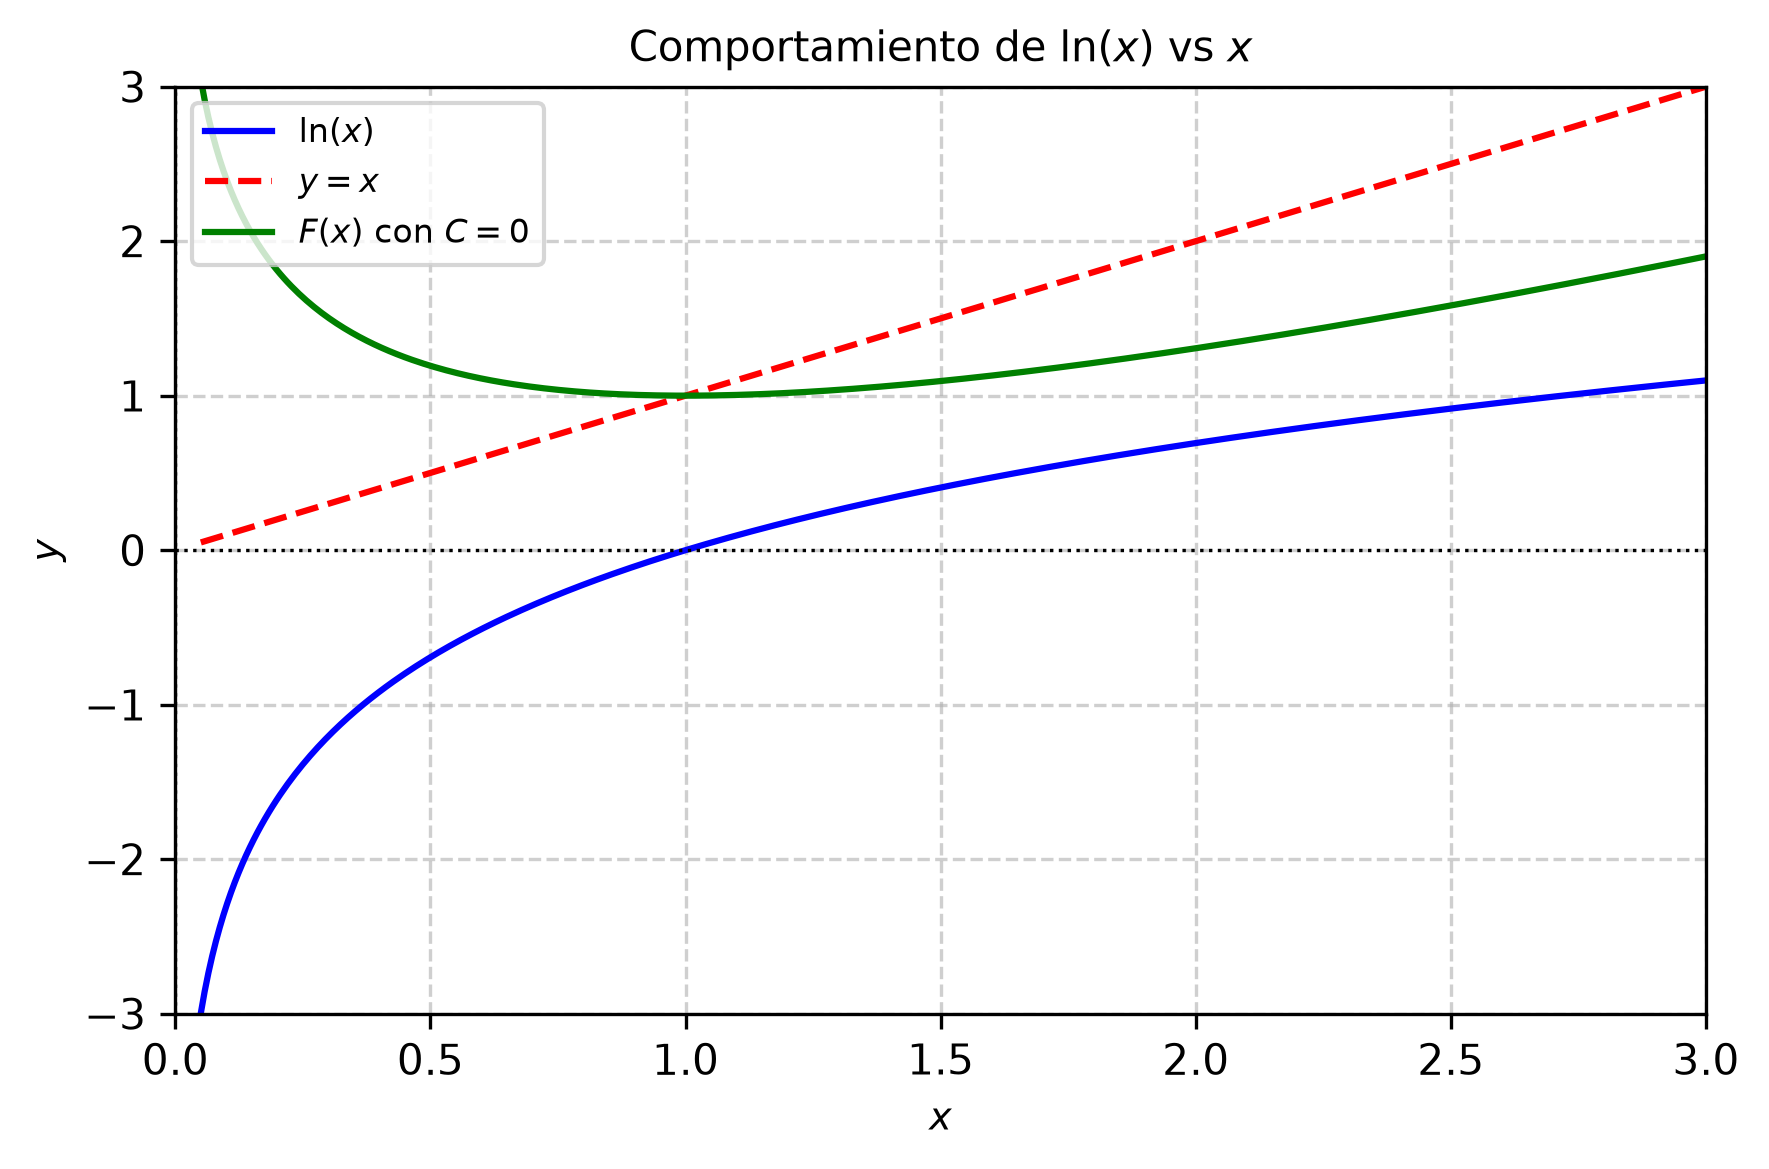
\includegraphics[width=\columnwidth]{semana_08/graficas/estesi.png}
    \caption{Representación gráfica de las funciones $\ln(x)$, $y=x$ y $f(x) = x - \ln(x)$ (Problema 02).}
    \label{fig:problema02}
\end{figure}
